%# -*- coding: utf-8-unix -*-
%%==================================================
%% chapter01.tex for SJTU Master Thesis
%%==================================================

%\bibliographystyle{sjtu2}%[此处用于每章都生产参考文献]
\chapter{实证分析}
\label{chap:analysis}

\section{数据选取和处理}

我们选取Wind提供的动力煤指数(ZCFI.WI)作为标的资产价格序列进行实证分析。动力煤指数由每个动力煤合约按照持仓额加权平均计算得出.选择动力煤指数而非动力煤主连合约作为标的资产价格序列的原因是,动力煤主连合约在主力合约切换时会发生跳价,无法计算此时的收益率及其波动率。

我们选取时间区间为2013年12月25日至2019年4月23日的动力煤指数日收盘价格数据,动力煤指数对数收益率的分布和描述性统计如下

\begin{figure}[htb]
  \centering
  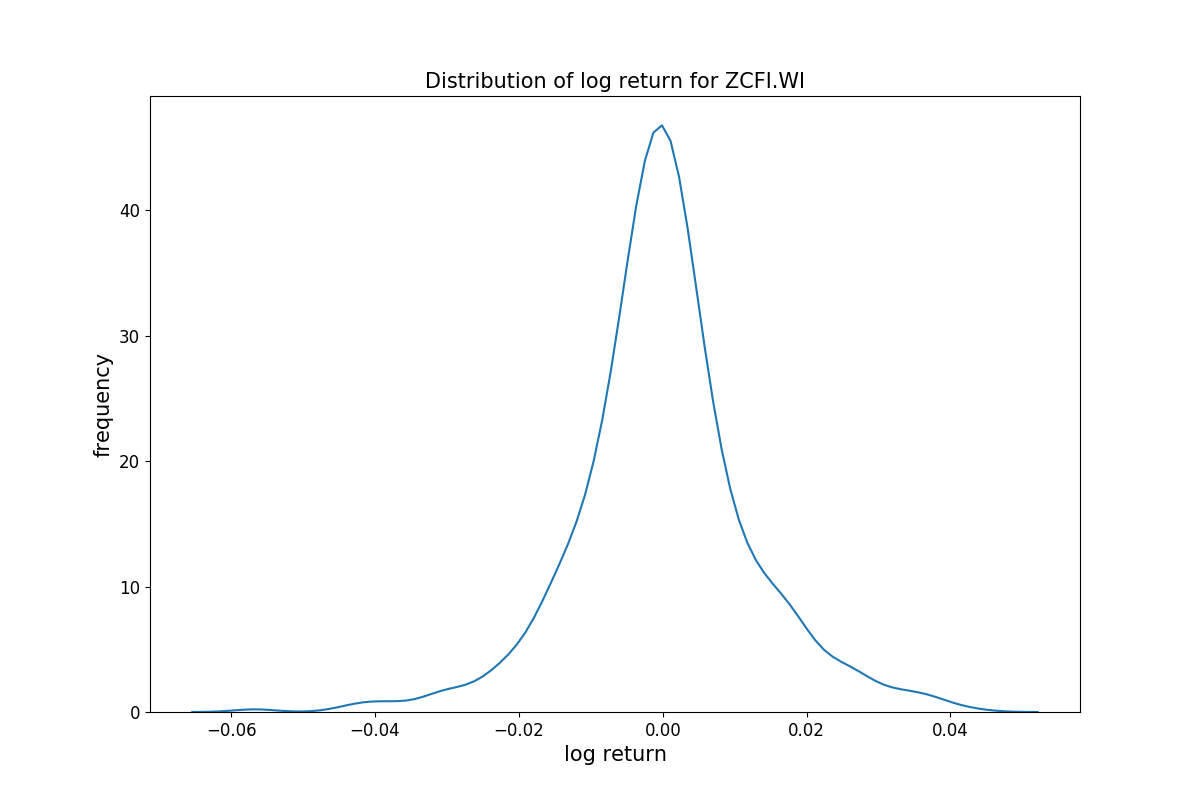
\includegraphics[width=12cm, height=8cm]{analysis/dist_ZCFI.png}
  \caption[这里将出现在插图索引中]
    {动力煤指数对数收益率分布}
  \label{fig:ZCFI_describe}
\end{figure}

\begin{table}[htbp]
  \centering
  \caption{动态对冲策略的$\mu$和$\sigma$}
  \label{tab:ZCFI_describe}
  \begin{tabular}{cc}
    \toprule
    统计量 & 值 \\
    \midrule
    mean & 4.20435E-05 \\
    std & 1.21309E-02 \\
    variance & 1.47159E-04 \\
    min & -5.67394E-02 \\
    max & 4.34607E-02 \\
    5\% & -1.96002E-02 \\
    25\% & -5.77001E-03 \\
    50\% & -1.99533E-04 \\
    75\% & 5.64455E-03 \\
    95\% & 2.06669E-02 \\
    iqr & 1.14146E-02 \\
    kurtosis & 2.09724E+00 \\
    skewness & -6.06696E-02 \\
    \bottomrule
  \end{tabular}
\end{table}

从图\ref{fig:ZCFI_describe}和表\ref{tab:ZCFI_describe}中可以看出,动力煤指数对数收益率存在着左偏的现象。经过Jarque-Bera检验,p值近似为0,说明动力煤指数对数收益率序列不服从正态分布,我们将在之后具体分析这一分布特点对其对冲结果的影响。

在动态对冲的实证研究中,需要确定计算Delta时使用的隐含波动率。我们将分别采用滚动计算的窗宽为60的历史波动率和滚动计算的$\beta$为0.94、最小窗宽为60的EWMA波动率作为这一波动率的估计,并比较两者对应的结果差异。两个波动率随时间变化的趋势如图\ref{fig:vol_ZCFI}。从图中可以看出,历史波动率相对于EWMA波动率更为平滑。计算得出历史波动率的均值约为0.18064,EWMA波动率的均值约为0.17919。

\begin{figure}[htb]
  \centering
  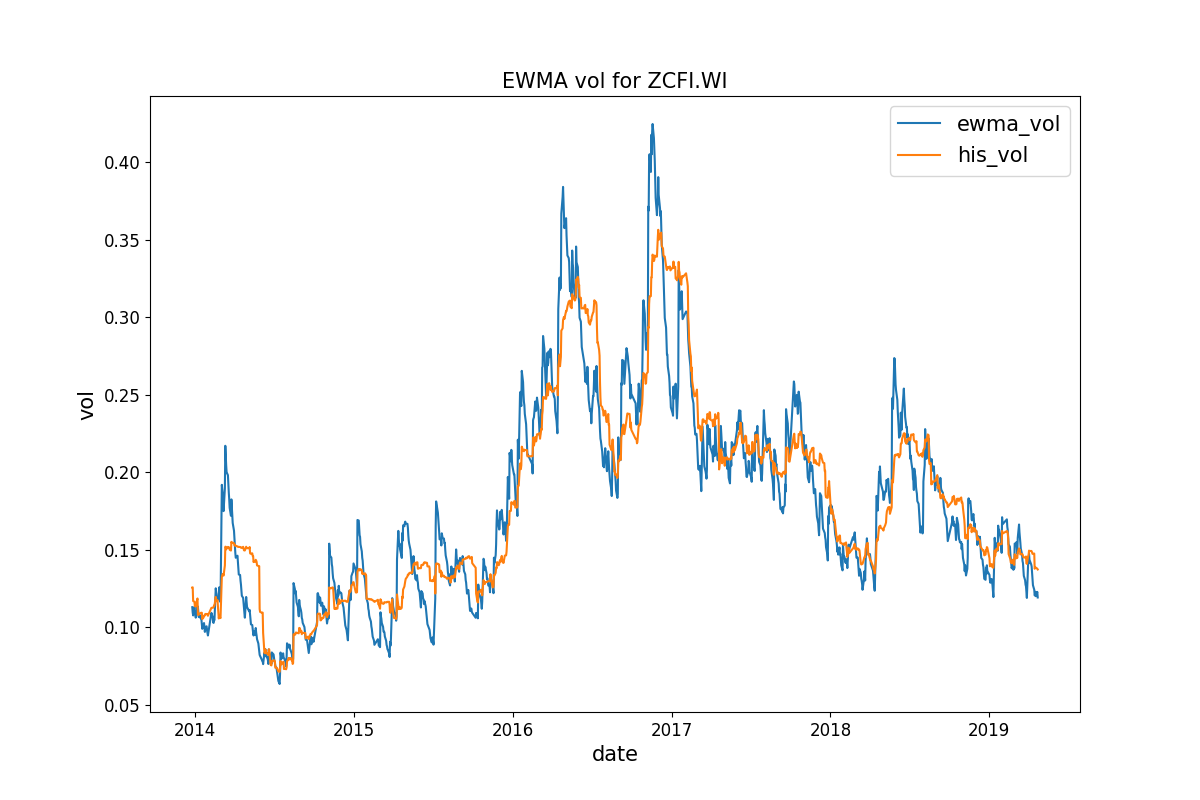
\includegraphics[width=12cm, height=8cm]{analysis/vol_ZCFI.png}
  \caption[这里将出现在插图索引中]
    {动力煤指数对数收益率的波动率}
  \label{fig:vol_ZCFI}
\end{figure}

\section{模型确立}

在上一章中,我们介绍了模拟研究中动态对冲操作的基本逻辑和评判指标。使用实际数据进行研究与模拟研究的原理类似,但是受数据特点的影响,我们在具体操作和结果评价上都有所调整。在动态对冲的具体操作中,我们在原数据上以60+1为窗宽滚动采样进行动态对冲策略的回测(第一个数据用于对冲组合的初始化)。在估计波动率时,我们使用第一个数据对应的历史波动率或EWMA波动率作为动态对冲中计算Delta时使用的隐含波动率。在确定行权价格时,我们使用第一个数据对应的动力煤指数价格为行权价。其他变量的设定与上一章相同。

在对冲结果的评价上,上一章以对冲成本为出发点,使用了期望对冲成本、相对对冲波动率和平均再平衡次数三个指标,也考察了对冲成本的波动率。本章由于滚动使用实际数据进行动态对冲分析,每个滚动窗口对应的隐含波动率均不相同,因此每段对应的期权理论价格也不相同,难以采用对冲成本进行评价。回顾第\ref{utility}小节,我们介绍并推导了年化对冲成本率的概念。年化对冲成本率是一个标准化的指标,一般为负值,可以用于不同隐含波动率、不同行权价格下对冲成本的比较。因此,我们在实证研究中,对于每一个滚动窗口下的对冲结果计算年化对冲成本率,最后计算年化期望对冲成本率、年化对冲成本率标准差、平均再平衡次数和对冲成本率偏度,作为对对冲结果的评价。我们将以交易费用为万分之五为例,计算固定时点动态对冲策略和固定Delta区间动态对冲策略在实际数据上的表现。

\section{固定时点动态对冲}

在实际数据上进行固定时点动态对冲,使用历史波动率的结果如下

\begin{table}[htbp]
  \centering
  \caption{使用历史波动率时固定时点动态对冲结果}
  \label{tab:fixed_time_5_his_vol_real}
  \begin{tabular}{cccccc}
    \toprule
    再平衡时间间隔 & 1 & 3 & 5 & 10 & 15 \\
    \midrule
    年化期望对冲成本率 & -0.21307 & -0.28222 & -0.30179 & -0.38262 & -0.58224 \\
    年化对冲成本率标准差 & 0.49910 & 0.60425 & 0.65314 & 0.66530 & 0.79351 \\
    平均再平衡次数 & 59.00000 & 19.00000 & 11.00000 & 5.00000 & 3.00000 \\
    对冲成本率偏度 & -1.26083 & -1.43039 & -1.82980 & -0.58411 & -0.72386 \\
    \bottomrule
  \end{tabular}
\end{table}

\begin{figure}[htb]
  \centering
  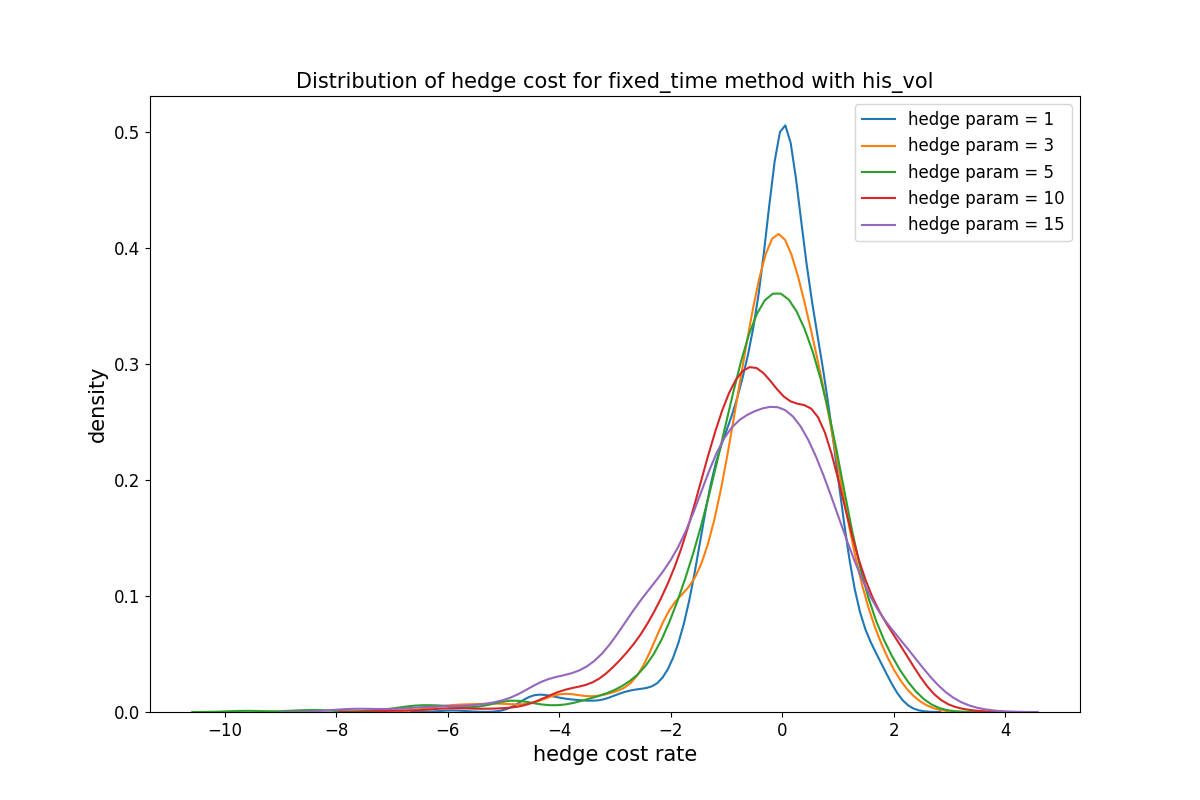
\includegraphics[width=12cm, height=8cm]{analysis/fixed_time_5_his_vol_real.png}
  \caption[这里将出现在插图索引中]
    {使用历史波动率时固定时点动态对冲年化对冲成本率分布}
  \label{fig:fixed_time_5_his_vol_real}
\end{figure}
使用EWMA波动率的结果如下

\begin{table}[htbp]
  \centering
  \caption{使用EWMA波动率时固定时点动态对冲结果}
  \label{tab:fixed_time_5_ewma_vol_real}
  \begin{tabular}{cccccc}
    \toprule
    再平衡时间间隔 & 1 & 3 & 5 & 10 & 15 \\
    \midrule
    年化期望对冲成本率 & -0.22197 & -0.29719 & -0.32270 & -0.42106 & -0.64521 \\
    年化对冲成本率标准差 & 0.50521 & 0.61185 & 0.66963 & 0.69798 & 0.85823 \\
    平均再平衡次数 & 59.00000 & 19.00000 & 11.00000 & 5.00000 & 3.00000 \\
    对冲成本率偏度 & -1.15463 & -1.30845 & -1.92706 & -0.56951 & -0.94468 \\
    \bottomrule
  \end{tabular}
\end{table}

\begin{figure}[htb]
  \centering
  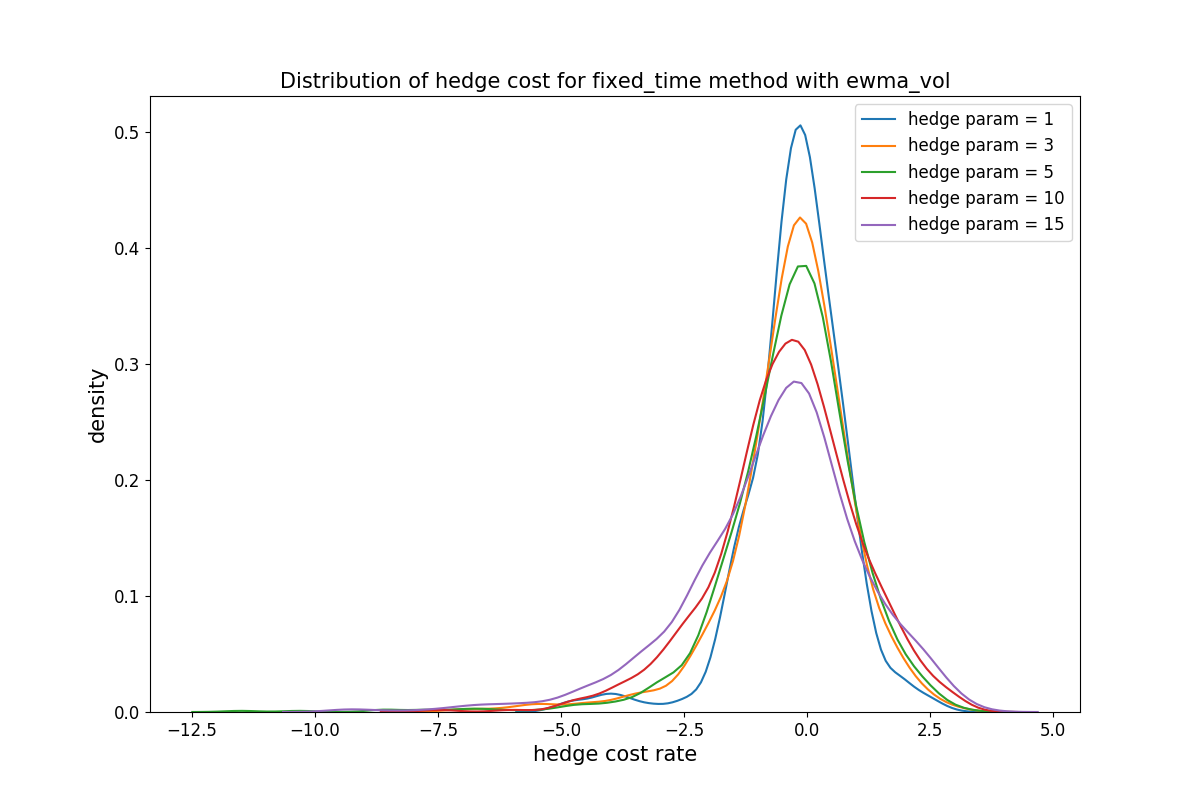
\includegraphics[width=12cm, height=8cm]{analysis/fixed_time_5_ewma_vol_real.png}
  \caption[这里将出现在插图索引中]
    {使用EWMA波动率时固定时点动态对冲年化对冲成本率分布}
  \label{fig:fixed_time_5_ewma_vol_real}
\end{figure}

首先,对比表\ref{tab:fixed_time_5_his_vol_real}和\ref{tab:fixed_time_5_ewma_vol_real},我们发现使用历史波动率时,年化期望对冲成本率的绝对值和年化对冲成本率标准差均低于使用EWMA波动率时的结果。年化期望对冲成本率较低是由于历史波动率的均值要高于EWMA波动率,因此使用历史波动率相当于是在复制了一个相对于EWMA波动率方法下有波动率溢价的期权。年化对冲波动率较低也是因为历史波动率的整体水平较高,在对冲时有一个更高的、与实际波动相关的时间价值来抵消一部分对冲成本,从而带来更低的在对冲成本上的波动。

\begin{table}[htbp]
  \centering
  \caption{模拟研究中的固定时点动态对冲结果}
  \label{tab:fixed_time_5_sim}
  \begin{tabular}{cccccc}
    \toprule
    再平衡时间间隔 & 1 & 3 & 5 & 10 & 15 \\
    \midrule
    年化期望对冲成本率 & -0.14990 & -0.10269 & -0.08800 & -0.07865 & -0.07967 \\
    年化对冲成本率标准差 & 0.21130 & 0.35532 & 0.45301 & 0.62981 & 0.76059 \\
    平均再平衡次数 & 59.00000 & 19.00000 & 11.00000 & 5.00000 & 3.00000 \\
    对冲成本率偏度 & -0.42441 & -0.38394 & -0.43164 & -0.54209 & -0.61634 \\
    \bottomrule
  \end{tabular}
\end{table}

之后,将实证分析的结果同模拟研究的结果进行对比。表\ref{tab:fixed_time_5_sim}展示了固定时点对冲的相应指标结果。我们发现,从绝对数值上看,实证分析的结果中的年化期望对冲成本率、年化对冲成本率标准差和对冲成本率偏度均明显高于模拟研究的结果。这可以从以下几个方面得到解释:首先,动力煤指数收益率的分布与正态分布相差较大,由此会带来对冲成本在分布上的差异;其次,由于实际数据的数据量有限,滚动进行的回测结果的数量无法达到与模拟研究相同级别的收敛程度;最重要的一点是,我们使用的是期初固定的波动率,可能无法准确地预测未来动力煤指数的实际波动率,并且由于卖出期权收益的不对称性,动力煤指数在波动率上的波动(volatility of volatility)也会给对冲带来额外的成本。

从相对数值上看,我们发现实证分析的结果中,年化对冲成本率标准差随平均再平衡次数的变化关系与模拟研究保持一致。然而,年化期望对冲成本率的这一关系差异较大。随着平均再平衡次数的减少,年化期望对冲成本率增加。这说明在实际对冲操作中,对冲不精确带来的损失远大于对冲频繁带来的额外交易成本。这也启示我们当不能够准确预测波动率时,可以通过更加频繁地再平衡操作来降低对冲成本。同时,由于不同再平衡次数下,实证分析结果的年化期望对冲成本率相差较大,对对冲成本率偏度的数值也有一定的影响。

\section{固定Delta区间动态对冲}

在实际数据上进行固定Delta区间动态对冲,使用历史波动率的结果如下

\begin{table}[htbp]
  \centering
  \caption{使用历史波动率时固定Delta区间动态对冲结果}
  \label{tab:fixed_interval_5_his_vol_real}
  \begin{tabular}{cccccc}
    \toprule
    Delta阈值 & 0.03 & 0.05 & 0.1 & 0.15 & 0.2 \\
    \midrule
    年化期望对冲成本率 & -0.22378 & -0.22533 & -0.30528 & -0.36488 & -0.52749 \\
    年化对冲成本率标准差 & 0.49734 & 0.49510 & 0.52071 & 0.55105 & 0.62216 \\
    平均再平衡次数 & 22.68119 & 15.58111 & 7.23487 & 4.22760 & 2.92333 \\
    对冲成本率偏度 & -1.17149 & -1.15062 & -0.73235 & -0.51298 & -0.38667 \\
    \bottomrule
  \end{tabular}
\end{table}

\begin{figure}[htb]
  \centering
  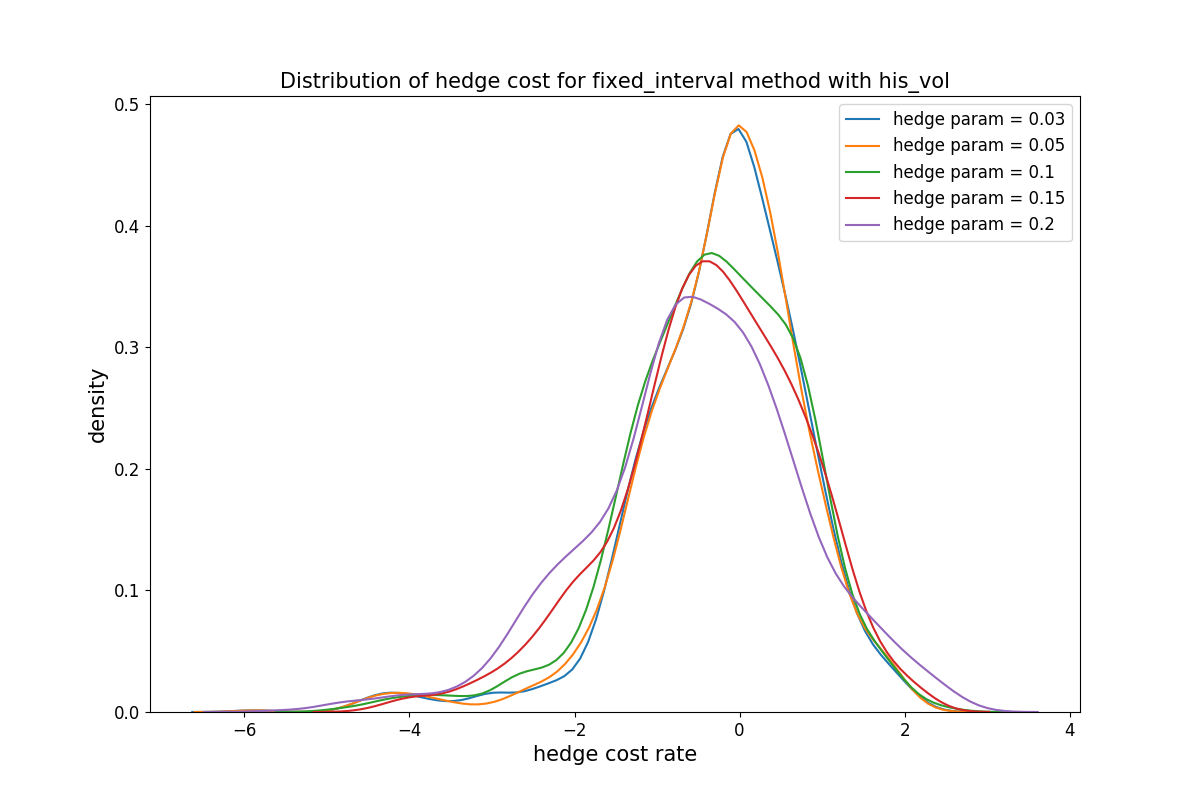
\includegraphics[width=12cm, height=8cm]{analysis/fixed_interval_5_his_vol_real.png}
  \caption[这里将出现在插图索引中]
    {使用历史波动率时固定Delta区间动态对冲年化对冲成本率分布}
  \label{fig:fixed_interval_5_his_vol_real}
\end{figure}
使用EWMA波动率的结果如下

\begin{table}[htbp]
  \centering
  \caption{使用EWMA波动率时固定Delta区间动态对冲结果}
  \label{tab:fixed_interval_5_ewma_vol_real}
  \begin{tabular}{cccccc}
    \toprule
    Delta阈值 & 0.03 & 0.05 & 0.1 & 0.15 & 0.2 \\
    \midrule
    年化期望对冲成本率 & -0.23541 & -0.22623 & -0.30755 & -0.41459 & -0.58979 \\
    年化对冲成本率标准差 & 0.50814 & 0.51192 & 0.53600 & 0.60002 & 0.67011 \\
    平均再平衡次数 & 22.58515 & 15.35916 & 7.29298 & 4.26715 & 2.93866 \\
    对冲成本率偏度 & -1.06379 & -1.03056 & -0.72411 & -0.50804 & -0.52199 \\
    \bottomrule
  \end{tabular}
\end{table}

\begin{figure}[htb]
  \centering
  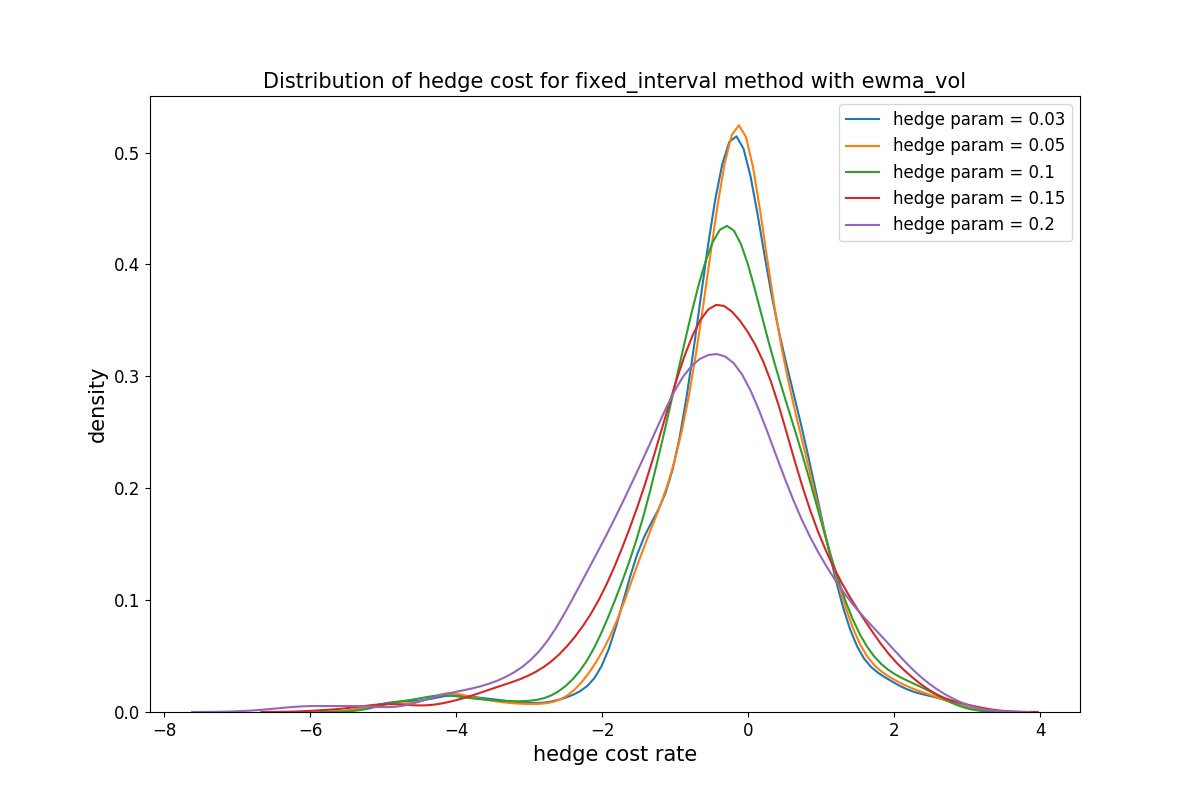
\includegraphics[width=12cm, height=8cm]{analysis/fixed_interval_5_ewma_vol_real.png}
  \caption[这里将出现在插图索引中]
    {使用EWMA波动率时固定Delta区间动态对冲年化对冲成本率分布}
  \label{fig:fixed_interval_5_ewma_vol_real}
\end{figure}

首先,对比表\ref{tab:fixed_interval_5_his_vol_real}和\ref{tab:fixed_interval_5_ewma_vol_real},结论与上一节类似。将本节结果与上一节的结果进行对比,我们发现固定Delta区间动态对冲的年化对冲成本率标准差整体上小于固定时点对冲,尤其是考虑到固定Delta区间动态对冲的平均再平衡次数明显较少,这说明在实际操作中,固定Delta区间动态对冲的再平衡操作更为高效。比较年化期望对冲成本率,固定Delta区间动态对冲策略下的结果从整体上看也明显较低。

然而,具体考察平均再平衡次数最高的结果,我们发现固定时点对冲策略的年化期望对冲成本率要低于固定Delta区间对冲策略的这一数值。这与上文提到的波动率估计不精确有关。在实际市场操作中,每日进行对冲操作最终可以获得更低的对冲成本,其带来的更为精确的对冲效果可以弥补额外的交易成本。

\begin{table}[htbp]
  \centering
  \caption{模拟研究中的固定时点动态对冲结果}
  \label{tab:fixed_interval_5_sim}
  \begin{tabular}{cccccc}
    \toprule
    Delta阈值 & 0.03 & 0.05 & 0.1 & 0.15 & 0.2 \\
    \midrule
    年化期望对冲成本率 & -0.13965 & -0.12642 & -0.10659 & -0.10273 & -0.09281 \\
    年化对冲成本率标准差 & 0.21840 & 0.23557 & 0.30927 & 0.40400 & 0.48942 \\
    平均再平衡次数 & 29.40321 & 20.23523 & 9.30451 & 5.20708 & 3.37050 \\
    对冲成本率偏度 & -0.34495 & -0.26154 & -0.16613 & -0.22670 & -0.19515 \\
    \bottomrule
  \end{tabular}
\end{table}

表\ref{tab:fixed_interval_5_sim}展示了模拟研究中固定时点对冲的相应对冲结果。将实证分析的结果同模拟研究的结果进行对比,结论与上一节较为类似,在此不再赘述。

\section{动态对冲策略和参数选择}

使用上一章提出的对冲得分指标,对实证分析的结果类似地做出评价,在此仅使用历史波动率下的结果。

\begin{figure}[htb]
  \centering
  \subcaptionbox{固定时点动态对冲}[12cm]
    {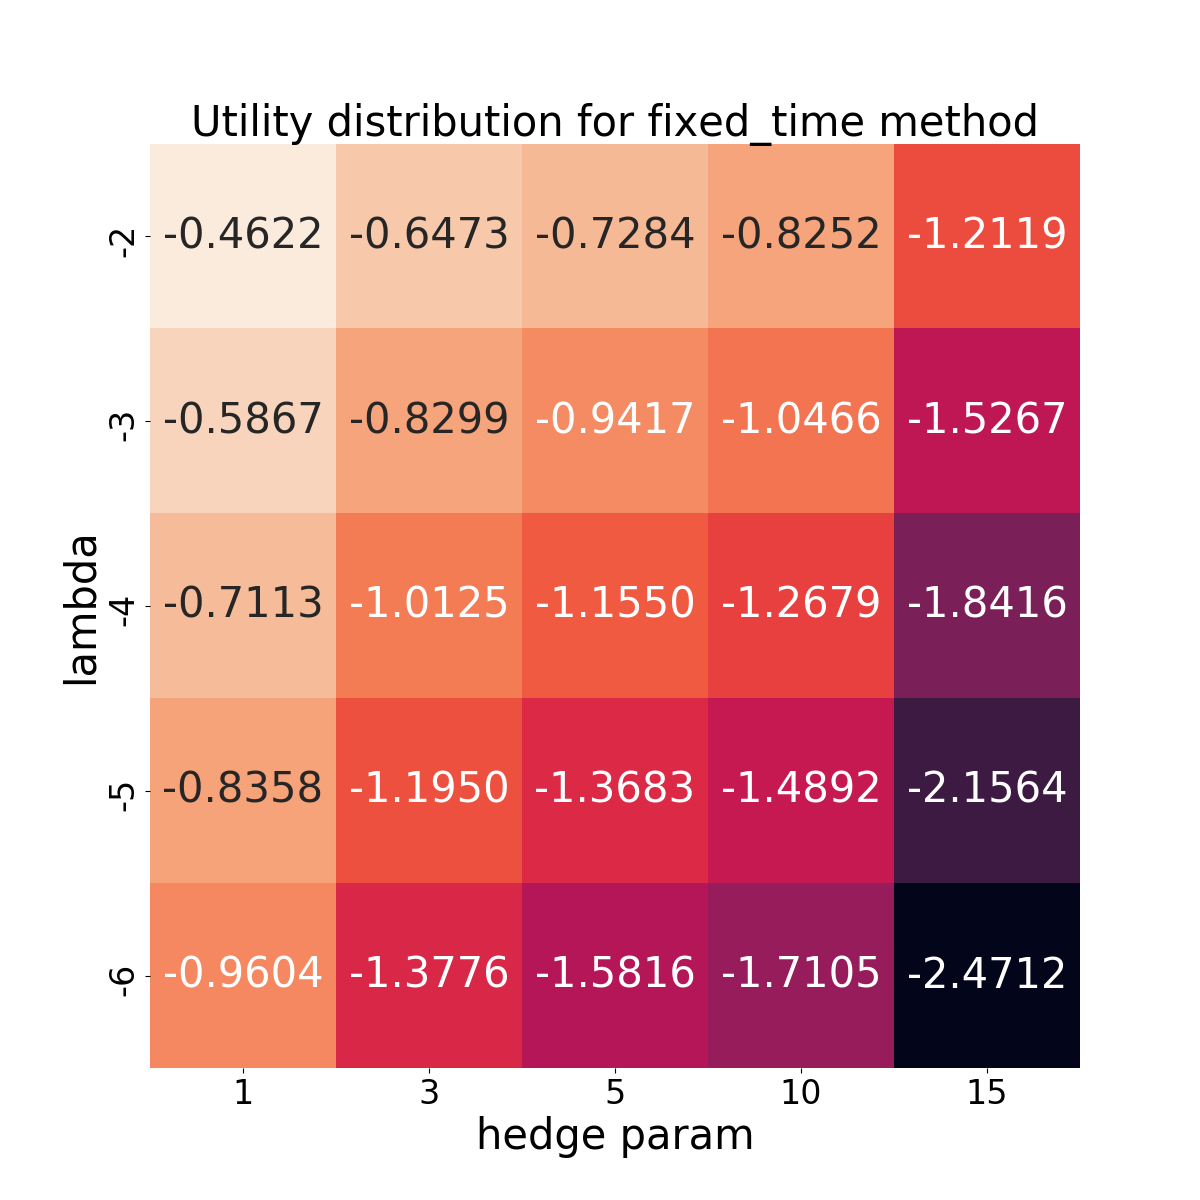
\includegraphics[width=7.5cm]{analysis/hedge_utility_real_fixed_time_his_vol.png}}
  \hspace{0.5cm}
  \subcaptionbox{固定Delta区间动态对冲}[12cm]
    {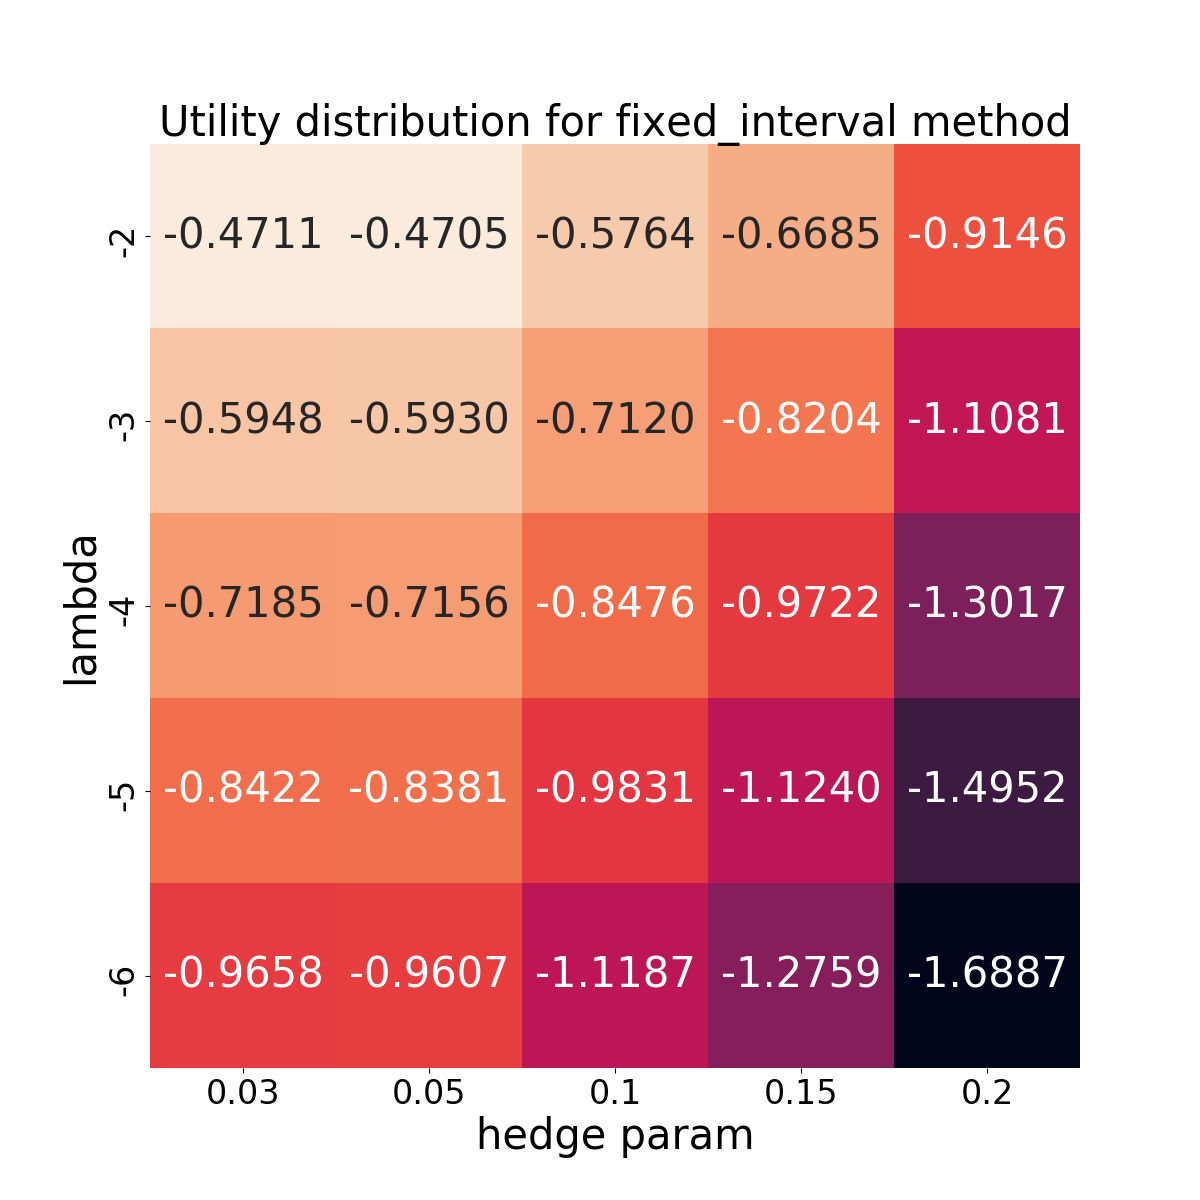
\includegraphics[width=7.5cm]{analysis/hedge_utility_real_fixed_interval_his_vol.png}}
    \caption[这里将出现在插图索引中]
    {均值-方差对冲得分}
  \label{fig:hedge_utility_real}
\end{figure}

两个策略的得分如图\ref{fig:hedge_utility_real}所示。从该图中可以看出,无论是固定时点对冲策略还是固定Delta区间对冲策略,在固定$\lambda$值时,对冲得分大致和对冲参数呈负相关关系。这一结论与模拟研究的结果类似,但是对于固定Delta区间策略,Delta阈值为0.05的结果要好于Delta阈值为0.03的结果。因此,在给定的参数范围内,对于固定时点对冲策略,场外期权交易商应当选择再平衡时间间隔为1天;对于固定Delta区间对冲策略,场外期权交易商应当选择Delta阈值为0.05。

横向对比固定时点对冲策略和固定Delta区间对冲策略,我们发现对于后四组结果,固定Delta区间对冲策略在对冲得分上的表现要明显好于固定时点对冲策略;而在第一组结果中,固定时点对冲策略较优。这说明从整体上看,固定Delta区间对冲策略还是要优于固定时点对冲策略。同时,比较再平衡时间间隔为1天和Delta阈值为0.05的结果,我们发现,随着风险厌恶系数绝对值的增加,两者对冲得分的差距逐渐缩小。注意到这一结果可能与动力煤指数的数据特点有关,是否具有普适性还需进一步研究。

基于以上实证分析,我们可以得出以下结论:场外期权交易商在对冲其动力煤看涨期权空头方向的暴露时,应当选择再平衡时间间隔为1天的固定时点动态对冲策略。

\section{本章小结}

本章使用动力煤指数的实际数据,对动态对冲进行了实证分析,并将结果与模拟研究的结果进行了比较。我们发现,在实际对冲操作中,与模拟研究不同,对冲不精确带来的损失远大于对冲频繁带来的额外交易成本,这说明我们应当采用对冲频率更高的动态对冲策略。这与动力煤指数收益率的分布特点有关,也取决于波动率预测的准确性。当不能够准确预测标的未来的波动率时,使用更高的对冲频率可以获得更好的对冲效果。基于这一分析,我们得出了在实际数据上,再平衡时间间隔为1天的固定时点动态对冲策略为最优对冲策略的结论。
